\section{Introduction}
\label{sec:introduction}

The Heavy Photon Search (HPS) prompt-resonance program is formulated in the minimal
visible dark-photon model, in which a new broken $U(1)_D$ gauge boson mixes
kinetically with the Standard-Model photon \cite{Holdom1986,EssigEtAl2011}. After
diagonalizing the gauge fields, the interaction terms relevant for the prompt
$A^\prime \rightarrow e^+e^-$ search can be written schematically as
\begin{equation}
\mathcal{L}
\supset
-\frac{1}{4}F_{\mu\nu}^{\prime}F^{\prime\mu\nu}
-\frac{\eps}{2}F_{\mu\nu}^{\prime}F^{\mu\nu}
\,+\,\frac{1}{2}m_{A^\prime}^{2}A_\mu^\prime A^{\prime\mu}
\,+\,\eps e J_{\mathrm{EM}}^\mu A_\mu^\prime .
\label{eq:dark-photon-lagrangian}
\end{equation}
Here $\eps$ is the kinetic-mixing parameter, $m_{A^\prime}$ is the dark-photon mass,
and $J_{\mathrm{EM}}^\mu$ is the ordinary electromagnetic current. In the low-mass
region considered here, the minimal visible model predicts a narrow prompt dielectron
resonance. Its natural width is negligible compared with the HPS detector resolution,
so the observed line shape is set by the experimental mass resolution
\cite{HPS2015DarkPhoton,HPS2016PromptLong}. This narrow-width regime makes a resonance
search well suited to the \SIrange{10}{300}{MeV} mass window: fixed-target
electroproduction can reveal a visibly decaying vector as a localized excess above the
smooth trident spectrum, in a coupling range that includes established dark-sector and
lepton-anomaly benchmarks.

In the fixed-target approximation relevant for HPS, prompt dark-photon production is
normalized to the radiative trident rate,
\begin{equation}
\sigma(e Z \rightarrow e Z A^\prime)
\simeq
\frac{3\pi \eps^2}{2\alpha_{\mathrm{EM}}}\,
m_{A^\prime}\,
\left.\frac{d\sigma_{\gamma^\ast}}{dm}\right|_{m=m_{A^\prime}},
\label{eq:ap-production}
\end{equation}
the analysis extracts a narrow signal yield from the smooth prompt $e^+e^-$ spectrum
and then converts that yield into a limit or best fit for $\eps^2$
\cite{EssigEtAl2011,HPS2015DarkPhoton,HPS2016PromptLong}. The physics interpretation
rests on the minimal prompt $A^\prime$ model and the radiative-trident normalization;
Gaussian-process regression (GPR) provides the statistical description of the smooth
background.

\subsection{Published HPS prompt-resonance searches}

The 2015 and 2016 engineering runs established the prompt-resonance analysis
used as the reference for this work. The 2015 search used
\SI{1170}{nb^{-1}} at \SI{1.056}{GeV} and covered \SIrange{19}{81}{MeV}.
Its smallest local $p$-value was $1.7\times10^{-3}$ at \SI{37.7}{MeV};
after accounting for the mass scan, the global $p$-value was 17\%
\cite{HPS2015DarkPhoton}. The 2016 search used \SI{10608}{nb^{-1}}
at \SI{2.3}{GeV} over \SIrange{39}{179}{MeV}. The smallest local
$p$-value, $6.38\times10^{-3}$ at \SI{94}{MeV}, corresponded to about
$1\sigma$ globally \cite{HPS2016PromptLong}. Neither search found evidence
for a prompt dark photon.

Figure~\ref{fig:published-hps-context} reproduces the published coupling limits
at their original confidence levels. The 2015 result is shown in its published
world-data context; the 2016 result includes its background-only expected bands.
Comparisons with the GPR analysis must account for the confidence construction, mass resolution and
radiative-fraction treatment; changing the background fit alone does not
make two limits directly equivalent.

\begin{figure}[H]
\centering
\begin{subfigure}[b]{0.48\linewidth}
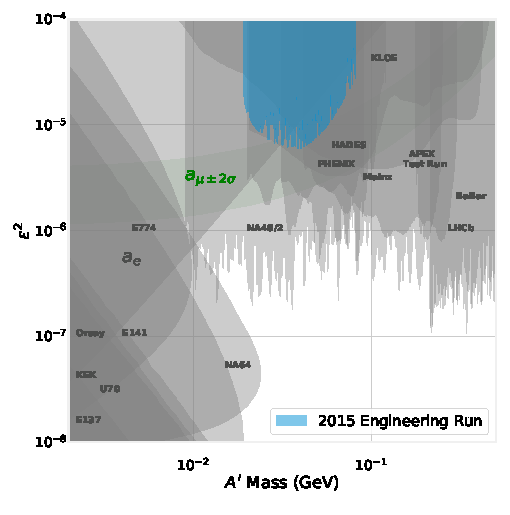
\includegraphics[width=\linewidth]{../figures/published_2015_limit_vector.pdf}
\caption{2015: published 95\% power-constrained limit.}
\end{subfigure}\hfill
\begin{subfigure}[b]{0.48\linewidth}
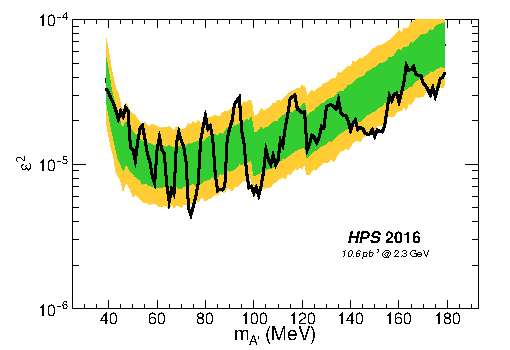
\includegraphics[width=\linewidth]{../figures/published_2016_limit_vector.pdf}
\caption{2016: published 95\% prompt limit and expected bands.}
\end{subfigure}
\caption{Published HPS prompt-search limits, reproduced from
Refs.~\cite{HPS2015DarkPhoton,HPS2016PromptLong} as vector figures.
The historical exclusions and lepton-anomaly region in (a) are those of the
2015 publication. In (b), green and yellow show the published 68\% and 95\%
background-only quantile ranges. Both panels retain the original analysis
and systematic treatment; no confidence-level rescaling is applied.}
\label{fig:published-hps-context}
\end{figure}

\subsection{Complementary prompt-visible constraints}

Figure~\ref{fig:hps-engineering-phase-space} places the prompt search in the
visible-dark-photon parameter space. The overview shows the published HPS engineering-run limits at 95\% CL and the
conditional combined projection at 90\% CL. The lower panels compare the
three-campaign and four-campaign projections on the same axes. The displaced
reach is shown separately because it uses a different search channel and a
simulation-based exposure assumption.

\begin{figure}[p]
\centering
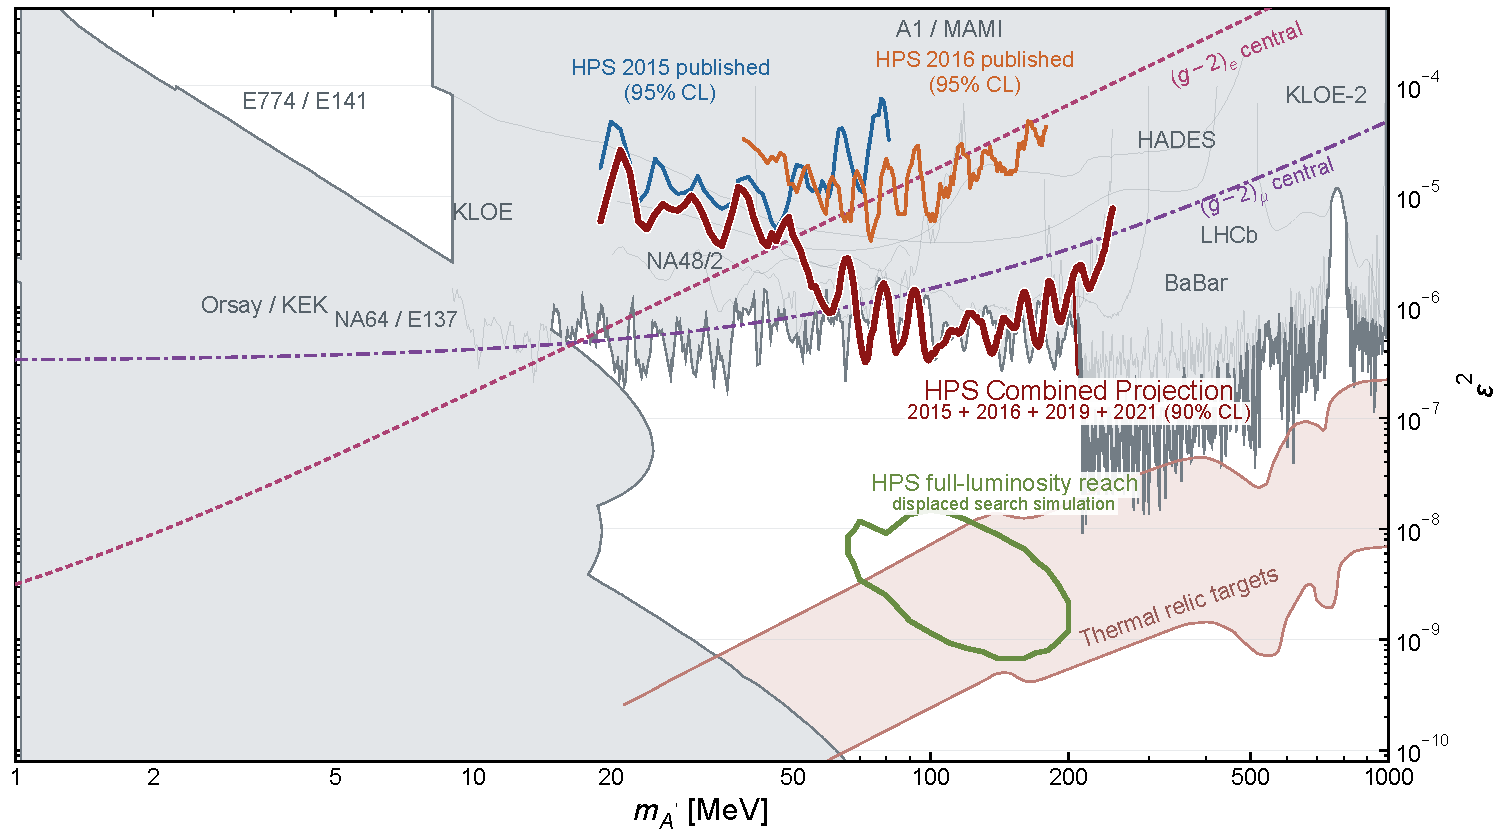
\includegraphics[width=\linewidth]{../figures/figure2_updated_overview.pdf}\\[3pt]
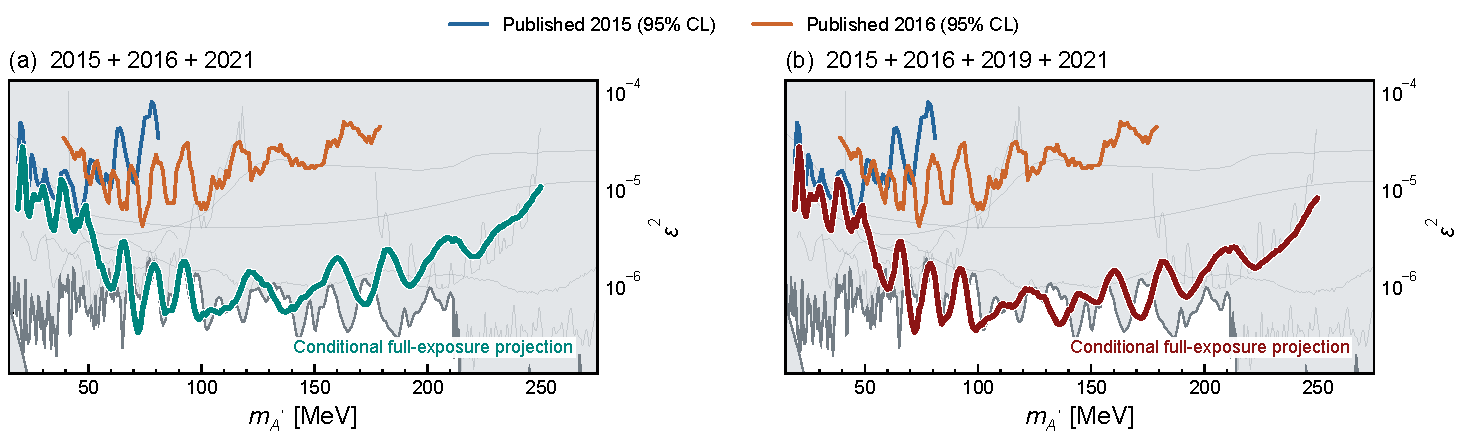
\includegraphics[width=\linewidth]{../figures/figure2_updated_panels.pdf}
\caption{Visible dark-photon parameter space. Top: archived exclusions,
published HPS 2015 and 2016 limits (95\% CL), the four-campaign prompt
projection (90\% CL), and the poster's simulated displaced full-luminosity
reach. The gray contours and thermal target are historical context, rather
than a complete 2026 survey; their sources and display conventions are
listed in Appendix~\ref{app:figure2-projections}. Lepton-anomaly lines show
central-value references only: $\Delta a_\mu=38\times10^{-11}$ (compatible
with zero) and $\Delta a_e\simeq0.34\times10^{-12}$
\cite{MuonWP2025,ElectronFan2023,AlphaMorel2020}.
(a) 2015+2016+2021; (b) 2015+2016+2019+2021. The prompt projections preserve
the current-sample structure and apply statistics-only density scaling to
full exposure. The 2019 dataset is a nominal 1\% sample with a 2021-response
proxy. These curves are conditional observed-equivalent projections;
they are not expected sensitivity curves or observed full-data exclusions.}
\label{fig:hps-engineering-phase-space}
\end{figure}

\subsection{Motivation for the present GPR analysis}

Gaussian-process regression is best viewed here as a modern form of
covariance-based interpolation. The historical starting point is kriging, developed in
mine-valuation and geostatistical applications by Krige and formalized by Matheron:
given observations of a smooth field at some locations, the task is to predict the
field elsewhere while carrying the uncertainty induced by finite sampling and spatial
correlation \cite{Krige1951,Matheron1963}. In a resonance search the coordinate is not
geographic position but invariant mass. The same statistical idea is useful because
the prompt trident continuum is smooth on the scale of the HPS mass resolution, while a
prompt $A^\prime$ would appear as a narrow localized excess. GPR replaces an explicit
closed-form background curve with a probability distribution over smooth functions,
specified by a mean and covariance kernel and conditioned on the observed training
bins outside the mass-dependent excluded window \cite{RasmussenWilliams2006}. For each
test mass, the practical output is therefore not only a background prediction in the
blinded window, but a correlated uncertainty on that prediction.

\begin{figure}[H]
\centering
\graphicorplaceholder{0.94\linewidth}{methodology_figs/gpr_intro_cartoon.png}
\caption{Cartoon of the per-test-mass GPR workflow. For each test mass, the GP is
trained on bins across the full mass range except for a narrow excluded window centered
on that mass. The trained GP predicts the posterior mean and covariance inside the
excluded window, where a narrow $A^\prime$-like signal hypothesis is overlaid only for
illustration.}
\label{fig:gpr-intro-cartoon}
\end{figure}

This viewpoint is attractive for HPS for the same reason emphasized in the 2017
high-energy-physics study of Frate \textit{et al.}: fixed empirical functions restrict
the background to a low-dimensional family, and discrepancies that are hidden by
statistical fluctuations can become limiting as luminosity grows or as the scan region
is widened \cite{FrateGP2017}. Figure~\ref{fig:frate-gp-vs-adhoc} reproduces three of
their comparison plots. In toy spectra built from ATLAS dijet data, the GP background
model maintains a near-unit goodness-of-fit scale and remains stable as the effective
luminosity increases, while the ad-hoc functional form degrades. The lesson for HPS is
not that a GP is assumption-free: the kernel, training exclusion, transform, and
length-scale bounds are all analysis choices. The benefit is that the smoothness
assumption is made explicit and propagated as a covariance, rather than being hidden in
a hand-selected analytic form.

\begin{figure}[p]
\centering
\begin{subfigure}[t]{0.88\linewidth}
  \centering
  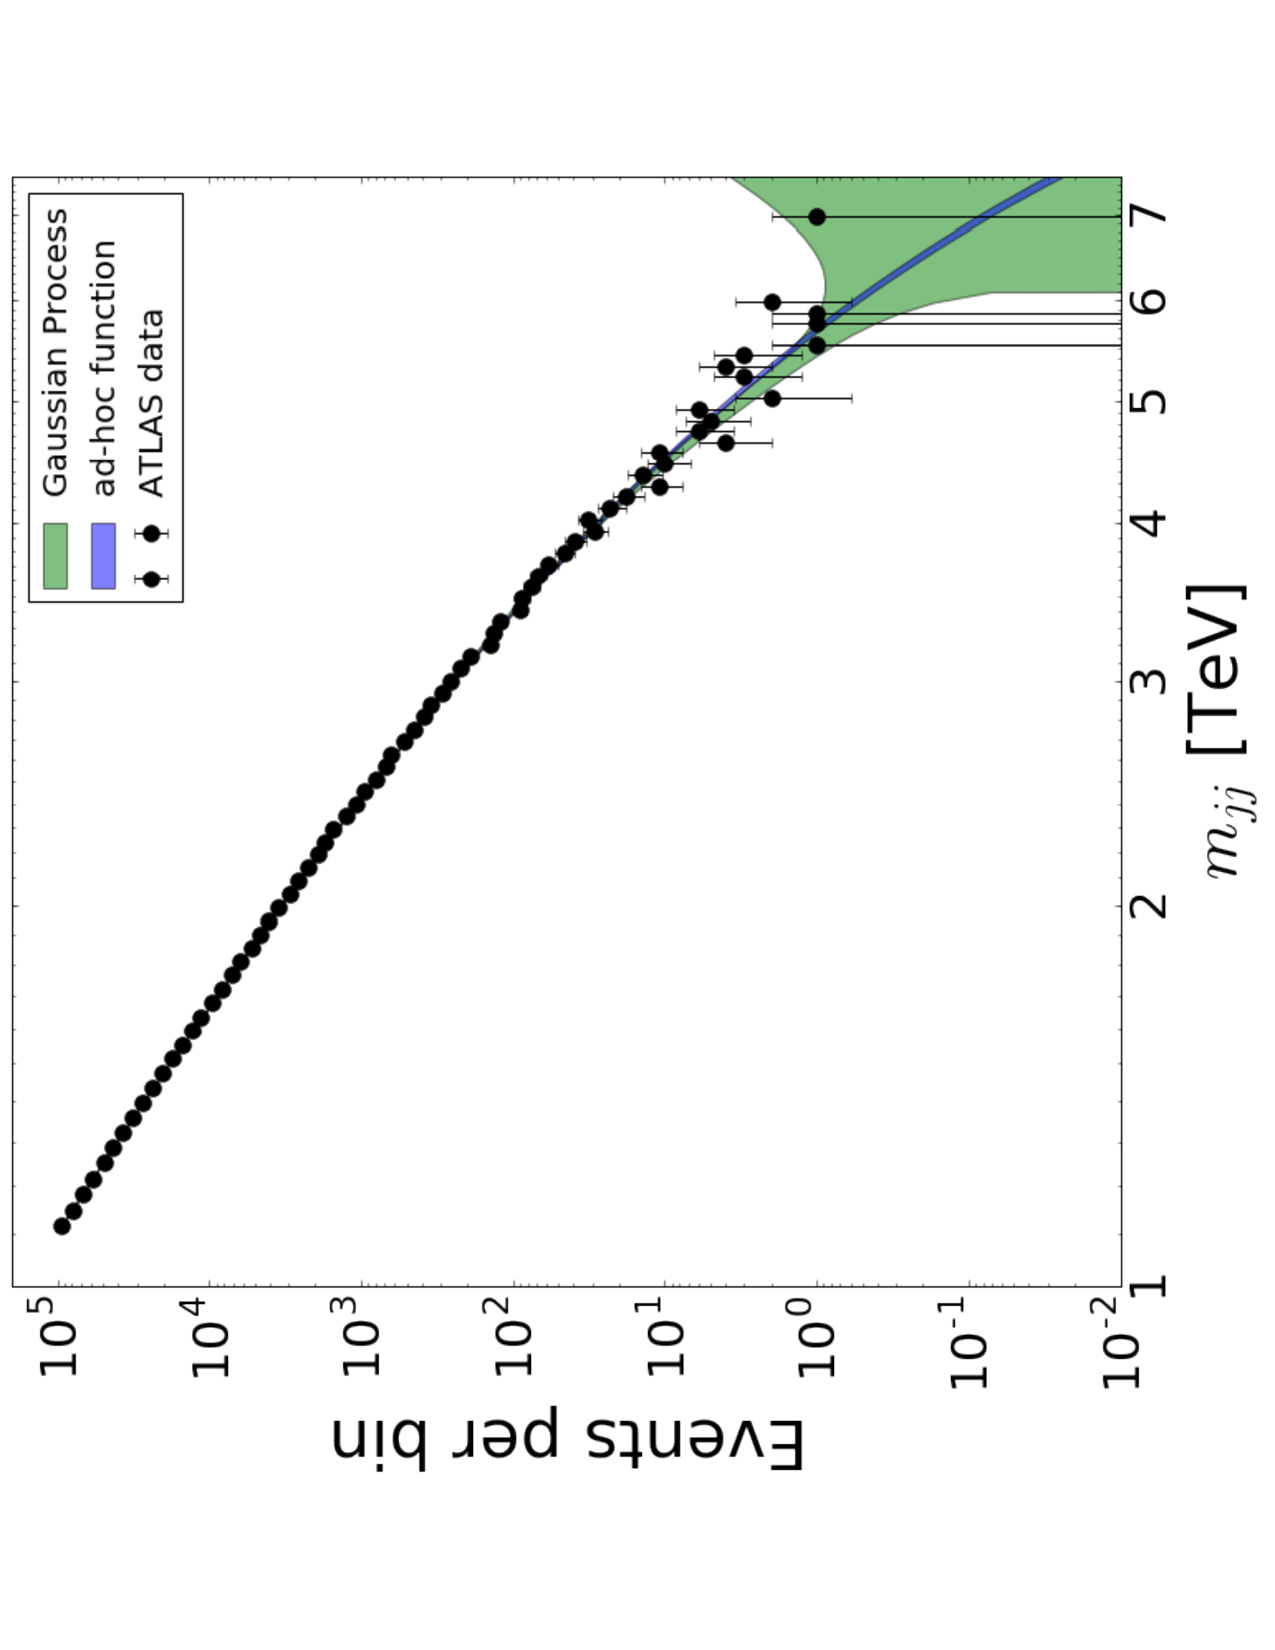
\includegraphics[width=0.58\linewidth,angle=-90]{external_figs/frate2017/FFGPonToys.pdf}
  \caption{Toy-spectrum mean and $\pm1\sigma$ background bands.}
\end{subfigure}

\vspace{0.8em}

\begin{subfigure}[t]{0.46\linewidth}
\centering
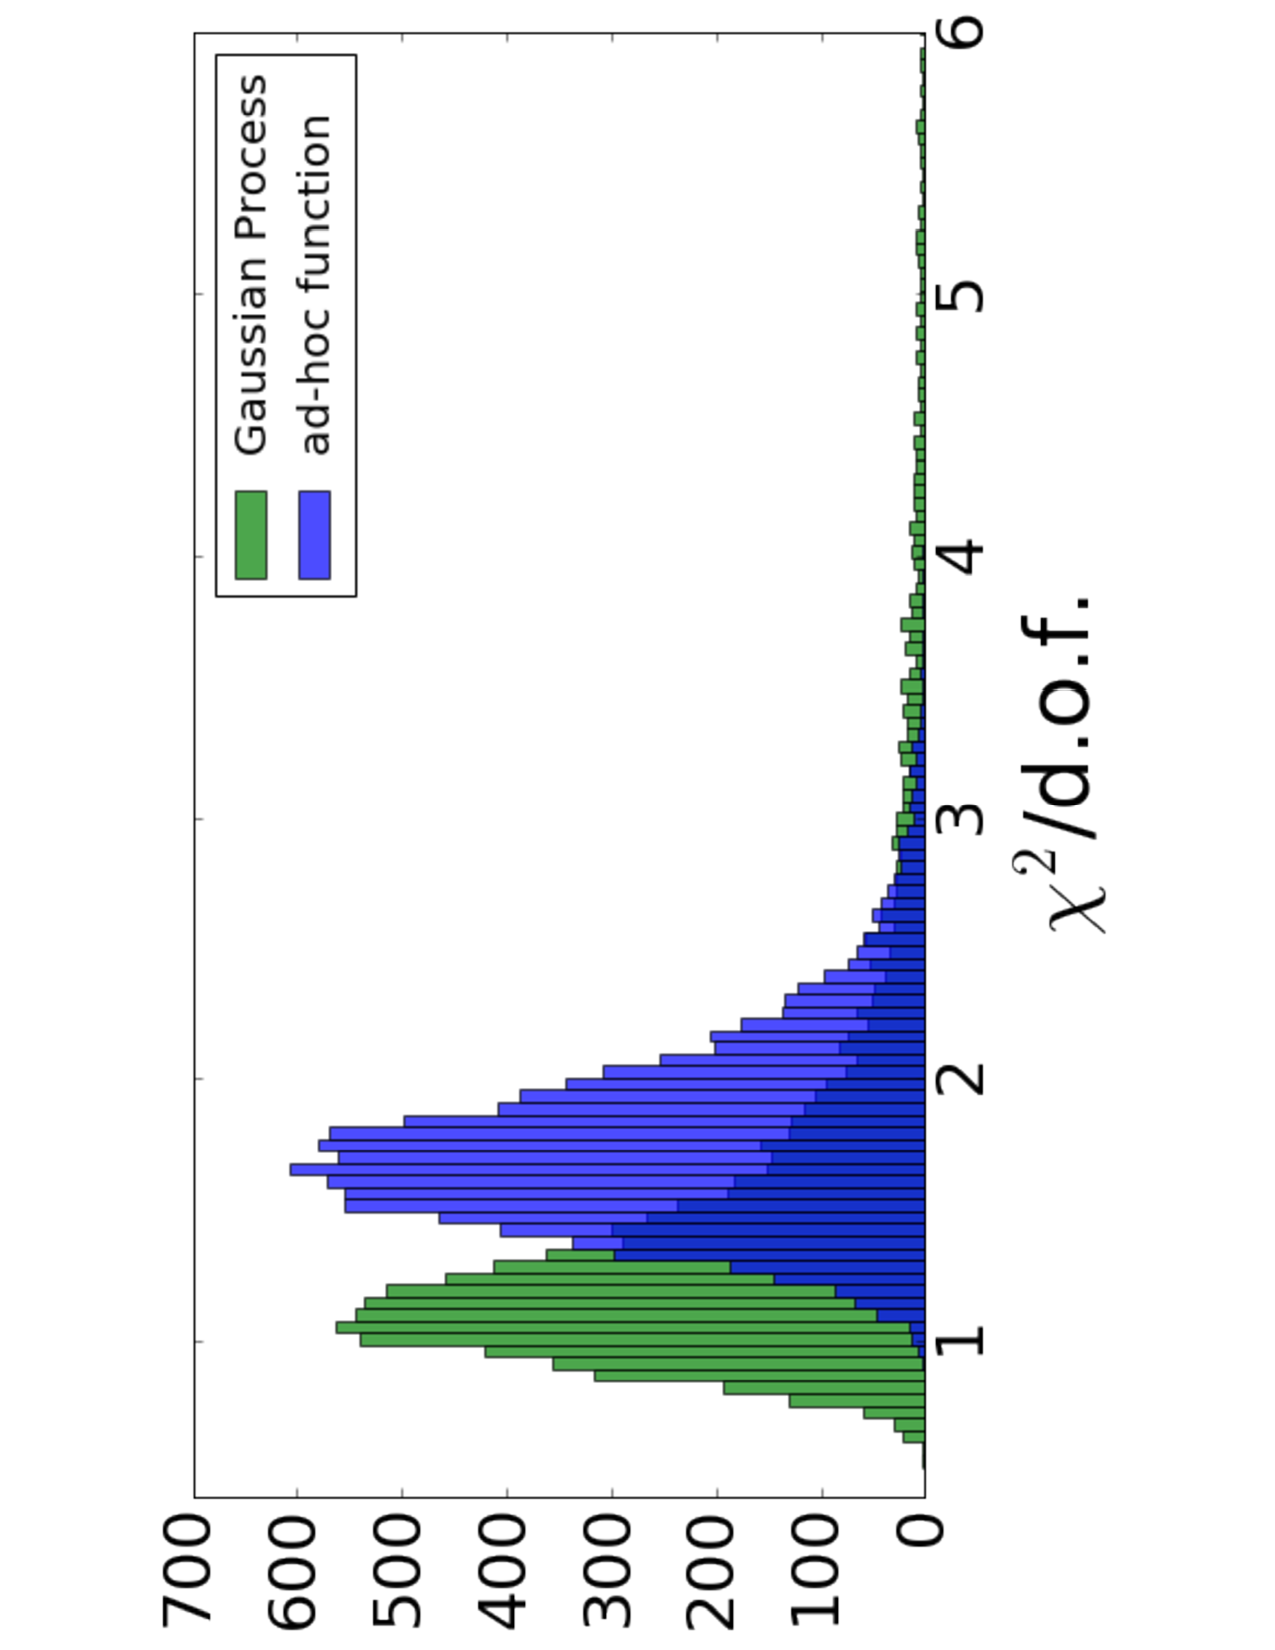
\includegraphics[width=0.76\linewidth,angle=-90]{external_figs/frate2017/chi2.pdf}
\caption{Toy goodness-of-fit distributions.}
\end{subfigure}
\hfill
\begin{subfigure}[t]{0.46\linewidth}
\centering
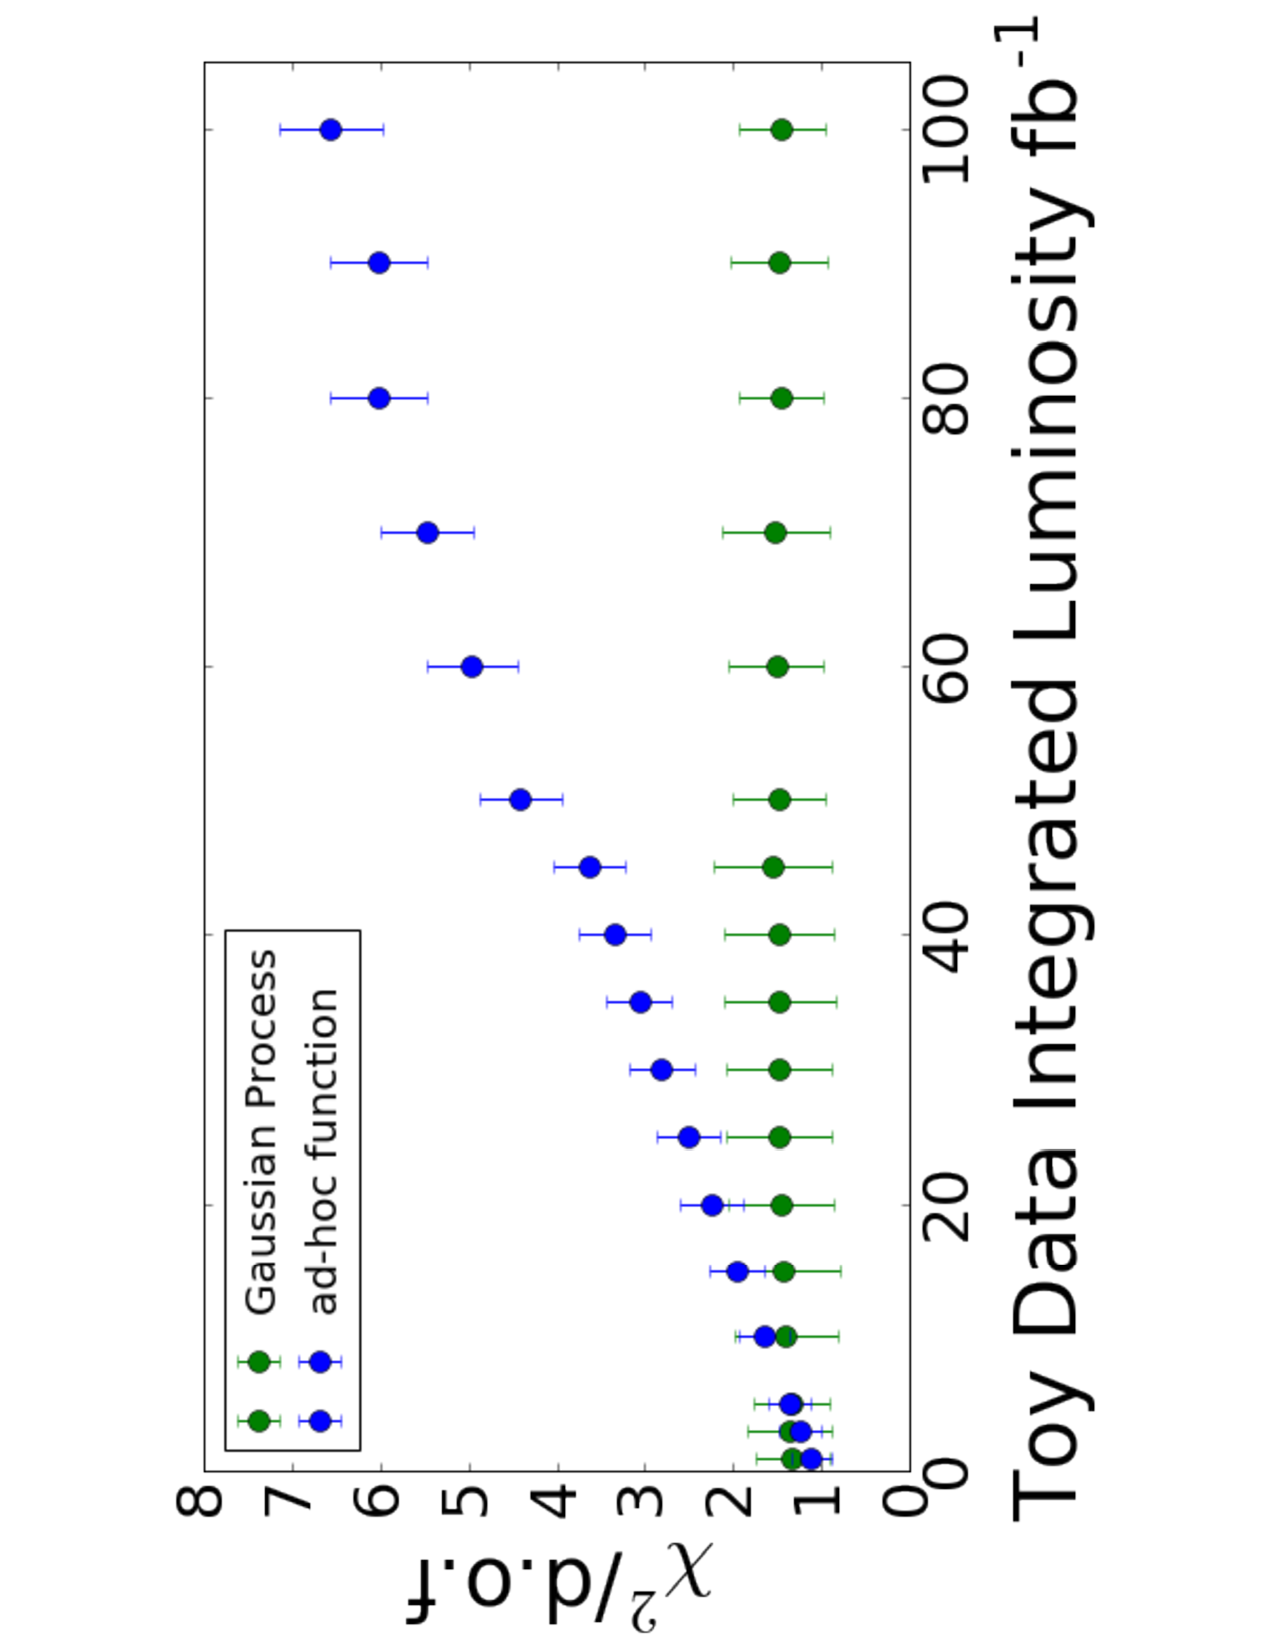
\includegraphics[width=0.76\linewidth,angle=-90]{external_figs/frate2017/lumivschi2.pdf}
\caption{Goodness of fit versus effective luminosity.}
\end{subfigure}
\caption{Methodological comparison between Gaussian-process and ad-hoc functional-form
background modeling reproduced from Ref.~\cite{FrateGP2017}. The panels show that, in
the 2017 dijet toy study, the GP retained an accurate smooth-background description
while the fixed functional form became increasingly strained as the effective
statistical precision improved.}
\label{fig:frate-gp-vs-adhoc}
\end{figure}

The later CMS-oriented GPR signal-extraction study by Gandrakota \textit{et al.}
provides the closest methodological bridge to the present implementation: choose a
kernel class, condition the GP on binned count data, compare candidate kernels against
the smooth background structure, and then separate a localized signal component from
the inferred background in a reproducible statistical workflow \cite{Gandrakota2023}.
The HPS analysis adopts that framework in a form matched to a fixed-target
prompt-resonance search. It trains the GP in log-mass/log-count space, removes the
test-mass window from training, ties the allowed length scale to the detector
resolution, converts the posterior prediction back into count space, and carries the
resulting mean vector and covariance matrix into the local profile likelihood. As
detailed in Section~\ref{sec:methodology}, GPR turns smooth-background interpolation
into an explicit probabilistic model that can be validated, profiled, and combined
across datasets.

Earlier HPS prompt searches used mass-window-specific background models,
window-by-window optimization, and a resonance extraction whose numerical behavior
depended on the local fit boundaries. Here, every mass hypothesis is assigned its own
GP fit on a fixed, dataset-specific support, with a narrow region around that hypothesis
excluded from training. The fit supplies a mean vector and covariance matrix for the
blinded bins. Signal extraction, local significance, modified-frequentist \CLs\ limits,
radiative-fraction conversion, and the shared-$\eps^2$ combination then follow within
one statistical framework.

This change is especially valuable for the present HPS program because one statistical
workflow must describe three campaigns with different mass ranges and detector
configurations. In v5 the tested signal hypotheses span \SIrange{19}{100}{MeV} for
2015, \SIrange{39}{180}{MeV} for 2016, and \SIrange{50}{250}{MeV} for 2021, while
the GP fit supports extend beyond those tested intervals to
\SIrange{14}{135}{MeV}, \SIrange{30}{210}{MeV}, and
\SIrange{36}{300}{MeV}, respectively. A stable GP model therefore matters both for
numerical smoothness and for carrying the same radiative-fraction and uncertainty
treatment across datasets without sacrificing narrow-resolution sensitivity. It also
motivates the combined analysis:
the minimal visible $A^\prime$ model predicts one common coupling $\eps^2$ at a given
mass, while each HPS run maps that coupling into a different expected signal yield
through its own integrated luminosity, acceptance, resolution, and radiative
normalization. The
statistical combination therefore treats $\eps^2$ as the shared parameter of interest
and multiplies the independent dataset likelihoods, profiling the dataset-specific
background nuisance parameters separately. In this common-parameter construction,
datasets with better local signal-to-background leverage carry more information, while
weaker channels still contribute correctly; the gain in sensitivity comes from adding
independent likelihood information for the same minimal-model signal rather than from
averaging separate limits after the fact.

\subsection{Scope of this note}

Version 5 consolidates the detector description, statistical method, validation
history and observed results for the proposed full-2021 unblinding review. The
current data comprise full 2015, full 2016 and the released 2021 10\% sample.
No additional 2021 events enter this document. The 2019 run enters only the explicitly identified Figure~\ref{fig:hps-engineering-phase-space}
projection; it does not enter the observed results in the results section.

The individual and combined fits use GP supports of 14--135, 30--210 and
36--300~MeV for 2015, 2016 and 2021. Earlier configurations are identified as
historical when they are needed to explain an analysis choice. Observed limits
use the bounded, piecewise-asymptotic 90\% \CLs{} construction with profiled
backgrounds. Pointwise expected-limit bands, empirical limit-tail diagnostics,
and the later conditional global-probability studies answer different questions
and are presented separately.

The calibration and global-significance studies examine how the results
depend on the assumed background spectrum. Appendix~\ref{sec:v5-history}
summarizes the development of the analysis.
